\documentclass[11pt]{article}
\usepackage[paper=a4paper,dvips,top=2.5cm,left=2.5cm,right=2.5cm,
    foot=2cm,bottom=2.5cm]{geometry}
\usepackage[utf8]{inputenc}
\usepackage{lipsum}
\usepackage{graphicx}
\usepackage{caption}
\usepackage{subcaption}
\usepackage{amsmath}

\begin{document}
\setlipsumdefault{1-10}
% %%%%%%%%%%%%%%%%%%%%%%%%%%%%%%%%%%%%%%%%%%%%%%%%%%%%%%%%%%%%%%%
% %%%%%%%%%%%%%%%%%%%%%REMERCIEMENTS
% %%%%%%%%%%%%%%%%%%%%%%%%%%%%%%%%%%%%%%%%%%%%%%%%%%%%%%%%%%%%%%%
% \part*{Remerciement}
% Je remercie....
% \pagebreak
% %%%%%%%%%%%%%%%%%%%%%%%%%%%%%%%%%%%%%%%%%%%%%%%%%%%%%%%%%%%%%%%
% %%%%%%%%%%%%%%%%%%%%%ENTREPRISE
% %%%%%%%%%%%%%%%%%%%%%%%%%%%%%%%%%%%%%%%%%%%%%%%%%%%%%%%%%%%%%%%
% \part*{Entreprise}
% Thales...
% \pagebreak
% %%%%%%%%%%%%%%%%%%%%%%%%%%%%%%%%%%%%%%%%%%%%%%%%%%%%%%%%%%%%%%%
% %%%%%%%%%%%%%%%%%%%%%INTRO
% %%%%%%%%%%%%%%%%%%%%%%%%%%%%%%%%%%%%%%%%%%%%%%%%%%%%%%%%%%%%%%%
% \part*{Introduction}
% Contexte
% -au sein de l'entreprise
% -au sein de l'equipe
% -au sein du domaine technique
% But du stage
% -resultats attendus
% -precedents resultats dans le domaine
% \pagebreak
% \part*{Deroulement}
% \section{Contrôle caméra et flux vidéo}

% \pagebreak
\section{Détection de personne}
Afin de mettre en place un suivi efficace des personnes, il faut commencer par être capable de détecter ces personnes. Il a donc fallu en premier lieu décider d'une méthode de détection de personnes adaptée à notre application. De nombreuses méthodes différentes existent dans ce domaine, mais l'environnement dans lequel nous effectuons cette détection fixe nos besoins:

-le suivi des personnes devant être fait en temps réel, il nous faut un algorithme suffisamment rapide pour ne pas avoir un impact trop important sur les performances du système complet;

-le fait que nous travaillons avec un caméra PTZ et que ce travail soit destiné à fonctionner dans des environnements variés élimine les méthodes de détection se basant sur un fond connu.\\
\\
Mon choix s'est porté sur une détection basée sur les histogramme de gradient orienté (HOG) pour son efficacité reconnue, sa rapidité et le fait que cet algorithme est suffisamment populaire pour pouvoir trouver des implémentations simples et des classifieurs entrainés sur des jeu de données correspondants à notre cas de figure.
L’implémentation utilisée est celle présente dans OpenCV sous le nom de 'HOGDescriptor' associé à un classifieur de type machines à vecteurs de support (SVM). Le descripteur utilisé est celui par défaut d'OpenCV pour les personnes.
\subsection{Principe de la détection HOG}
Cette méthode a été présentée par Navneet Dalal et Bill Triggs en 2005 dans le papier 'Histograms of Oriented Gradients for Human Detection'.
Elle consiste en une série d'étapes illustrées dans la figure~\ref{fig:hog_topo}.
% \begin{figure}[!ht]
%     \label{fig:hog_topo}
%     \centering
% 	    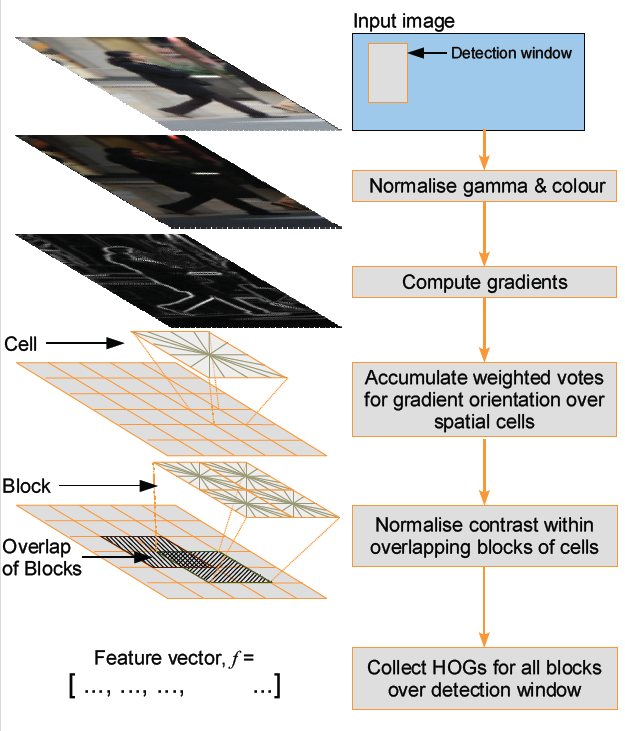
\includegraphics[width=0.7\textwidth]{hog_topo.png}
% 	    \caption{Illustration HOG+SVM}
% \end{figure}

%%%%%%%%%%%%%%%%%%%%%%%%%%
\subsection{Descripteur HOG}
Dans cette méthode, le descripteur (nommé HOG-D) est basé sur un ensemble d'histogrammes de gradient orientés. Le calcul de ces histogrammes est décris ci-dessous:
\subsubsection{Découpage de l'image}
Le descripteur est calculé pour une image de 64x128 pixels, ces dimensions représentent les proportions choisi pour une personne. C'est également la résolution utilisée pour la base d'image 'INRIA Person Dataset' réunie pour tester cette méthode.
Cette image est découpée en cellules de 8x8 pixels, ces cellules sont utilisées pour faire des blocs de 2x2 cellules (16x16 pixels). Les blocs se recoupent à 50\%, ce qui donne un total de 7 blocs en largeur par 15 blocs en hauteur. On a donc un total de 105 blocs contenant chacun 4 cellules.
\\
\begin{figure}[!ht]
\centering
\begin{subfigure}{.3\textwidth}
  \centering
  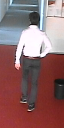
\includegraphics[width=.8\linewidth]{person.png}
  \caption{Image d'origine}
  \label{fig:kernel_sx}
\end{subfigure}%
\begin{subfigure}{.3\textwidth}
  \centering
  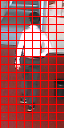
\includegraphics[width=.8\linewidth]{crossed.png}
  \caption{Découpage en cellules}
  \label{fig:kernel_sy}
\end{subfigure}
\begin{subfigure}{.3\textwidth}
  \centering
  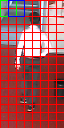
\includegraphics[width=.8\linewidth]{block.png}
  \caption{Deux premiers blocs}
  \label{fig:kernel_sy}
\end{subfigure}
\caption{Découpage de l'image en blocs et en cellules}
\label{fig:kernels}
\end{figure}

\subsection{Calcul des gradients}
Les gradients orientés sont calculés à l'aide de deux gradients pour chaque pixel: un gradient horizontal et un gradient vertical notés $S_{x}$ et $S_{y}$ tel que:
\[S_{x(i,j)}=I_{(i+1,j)}-I_{(i-1,j)}\]
\[S_{y(i,j)}=I_{(i,j+1)}-I_{(i,j-1)}\]
Les noyaux utilisés pour calculer ces deux valeurs sont illustrés dans la fig ???
\\
\begin{figure}[!ht]
\centering
\begin{subfigure}{.3\textwidth}
  \centering
  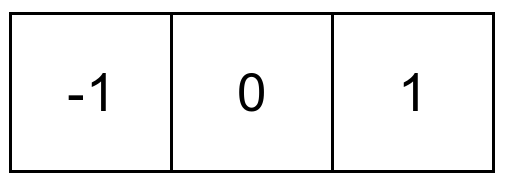
\includegraphics[width=.6\linewidth]{Sx.png}
  \caption{$Sx$}
  \label{fig:kernel_sx}
\end{subfigure}%
\begin{subfigure}{.3\textwidth}
  \centering
  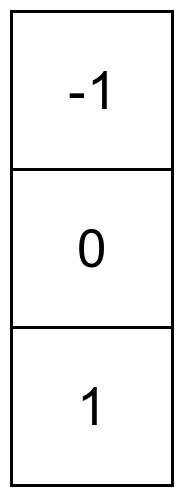
\includegraphics[width=.2\linewidth]{Sy.png}
  \caption{$Sy$}
  \label{fig:kernel_sy}
\end{subfigure}
\caption{Noyaux des gradients horizontaux (a) et verticaux (b)}
\label{fig:kernels}
\end{figure}
\\
Blabla le gradient orienté est représenté par le vecteur: 
$\bar{S}=\begin{pmatrix}S_{x}\\S_{y}\end{pmatrix}$
Les caractéristiques du gradient sont donc:\\
\[\|S\|=\sqrt{S_{x}^{~2}+S_{y}^{~2}}\]
\[\Omega_{S} = arctan(\frac{S_{y}}{S_{x}})\]

\subsection{Calcul des histogrammes}
Pour chaque cellule, un histogramme est obtenue grâce à la somme pondérée des orientations des gradients 
%%%%%%%%%%%%%%%%%%%%%%%%%%

\subsection{SVM}
type de classifieur... machine learning toussa toussa

\subsection{Paramètres et traitement des rectangles}
-paramètres utilisés et pourquoi
-gestion des rectangles multiples

\subsection{Resultat obtenues}
-10FPS
-pratiquement aucun faux positifs
(géré par le tracking sisi)
-pratiquement complet niveau detection face/dos
(géré aussi maggle)
-lacune: detection de profil

% \section{Suivi de personnes}
% \section{Decision de flight plan de caméra}
% \section{Detection de visage}
% \pagebreak
% \part*{Resultats et amélioration}
% \pagebreak
% \part*{Conclusion}
% \pagebreak

\end{document}